\documentclass[conference]{IEEEtran}
\IEEEoverridecommandlockouts
\usepackage{cite}
\usepackage{amsmath}
\usepackage{newtxtext,newtxmath}
\usepackage{graphicx}
\usepackage{booktabs}
\usepackage{multirow}
\usepackage{xcolor}
\usepackage{tikz}
\usetikzlibrary{arrows.meta,positioning,fit,calc}
\usepackage[hidelinks]{hyperref}

\definecolor{vizblue}{HTML}{2A78D6}
\definecolor{vizblueL}{HTML}{EEF4FC}
\definecolor{vizgray}{HTML}{F3F2EE}
\definecolor{vizink}{HTML}{52514E}

\begin{document}

\title{A Leakage-Aware Cascaded Learning Framework for Pan-Cancer Organ-of-Origin, Stage, and Survival Prediction from Routine Clinical Data}

\author{
\IEEEauthorblockN{Pravesh Shrivastava}
\IEEEauthorblockA{\textit{Department of \{Department Name\}} \\
\textit{\{Institution Name\}}\\
\{City\}, India \\
\{email address\}}
\and
\IEEEauthorblockN{Aniket Nawkar}
\IEEEauthorblockA{\textit{Department of \{Department Name\}} \\
\textit{\{Institution Name\}}\\
\{City\}, India \\
\{email address\}}
}

\maketitle

\begin{abstract}
Determining a tumour's organ of origin, anatomic stage and prognosis usually requires molecular assays, digitised pathology or complete TNM staging. We investigate how far these questions can be answered from routinely recorded structured clinical variables alone. Using 9,523 patients from The Cancer Genome Atlas (TCGA), spanning 32 projects grouped into 23 organ classes, we propose a leakage-aware cascaded framework in which an organ model feeds a stage model (AJCC I--IV, trained without TNM fields), and both feed a survival model that outputs vital status with a risk score. Structural missingness is encoded explicitly, all preprocessing is fitted within training folds, and eight classifiers, including XGBoost, LightGBM and CatBoost, are compared under nested, repeated stratified cross-validation with corrected resampled $t$-tests. Logistic regression identified the organ of origin with 94.4\% accuracy and a macro-F1 of 0.937 (0.955 on records with a recorded morphology code), significantly outperforming all tree-based ensembles and $k$-nearest neighbours. Stage prediction without TNM reached a macro-F1 of 0.505, with 84.7\% of predictions within one stage; including TNM inflated this to 0.90--0.95 through leakage. CatBoost achieved the best survival discrimination (AUC 0.847, Brier score 0.142), with logistic regression close behind (AUC 0.838, Brier score 0.146). Ablation attributed 28.4 macro-F1 points of organ performance to the ICD-O-3 morphology code, and cascading predicted rather than true organ labels caused no measurable loss. Interpretable linear models over routine variables therefore provide a strong, low-cost baseline for pan-cancer decision support, with gradient boosting adding a small gain only for survival.
\end{abstract}

\begin{IEEEkeywords}
cancer classification, clinical decision support, data leakage, machine learning, nested cross-validation, survival prediction, TCGA
\end{IEEEkeywords}

\section{Introduction}
Three questions dominate the first clinical encounter after a tumour is found: \emph{where} the cancer originated, \emph{how far} it has progressed, and \emph{what} the patient's outlook is. The primary site determines the treatment pathway and remains unresolved for patients with cancer of unknown primary~\cite{varadhachary2014}; anatomic stage under the AJCC system drives therapy selection and prognosis~\cite{amin2017}; and an individual risk estimate supports counselling and follow-up planning. Machine learning (ML) has been applied to each of these questions~\cite{cruz2006,kourou2015}, but the most accurate tissue-of-origin systems depend on transcriptomes~\cite{grewal2019}, targeted DNA panels~\cite{penson2020}, whole-genome mutation patterns~\cite{jiao2020}, or digitised whole-slide images~\cite{lu2021}. These inputs are costly and are frequently unavailable in resource-limited settings.

In contrast, a small set of structured variables---age, sex, the ICD-O-3 morphology code~\cite{fritz2000}, stage and TNM fields, treatment, and recurrence---is recorded for nearly every patient in routine care. How much clinical information these variables carry, when modelled jointly across many cancer types, has received comparatively little attention. Two methodological hazards make the question harder to answer than it appears. First, clinical tables contain fields that directly encode the outcome (for example, TNM categories \emph{define} AJCC stage), so careless feature selection produces inflated accuracy through data leakage~\cite{kaufman2012,kapoor2023}. Second, single train--test splits and model selection on the evaluation data give optimistic and unstable estimates~\cite{cawley2010}, and the claimed superiority of complex learners over logistic regression frequently disappears under rigorous validation~\cite{christodoulou2019}.

This paper addresses these gaps with a cascaded, leakage-aware framework evaluated on 9,523 patients from The Cancer Genome Atlas (TCGA). Our contributions are:
\begin{itemize}
\item a three-stage cascade that predicts organ of origin (23 classes), AJCC stage (I--IV), and vital status from routine clinical variables only, treating structural missingness as an informative category;
\item a leakage-controlled benchmark of eight classifiers, including three gradient-boosting libraries, under nested, repeated stratified cross-validation with corrected significance tests;
\item a feature-group ablation that quantifies which clinical variables drive organ prediction;
\item an analysis of error propagation through the cascade, showing that predicted organ labels can replace true labels without measurable loss; and
\item a calibration analysis of the survival risk score and a lightweight web deployment of the full pipeline.
\end{itemize}

\section{Related Work}
\subsubsection*{Tumour-type prediction}
Pan-cancer molecular profiling of about 10,000 TCGA tumours showed that most data types cluster primarily by cell of origin~\cite{hoadley2018}, which motivated classifiers of tissue of origin. SCOPE applied a neural network to whole transcriptomes~\cite{grewal2019}; Penson \emph{et al.} predicted 22 tumour types from a clinical sequencing panel with about 74\% accuracy~\cite{penson2020}; Jiao \emph{et al.} reached 91\% on 24 types from passenger mutations~\cite{jiao2020}; and TOAD inferred origin from routine histology slides~\cite{lu2021}. All four require molecular assays or slide digitisation. Our work asks how far structured clinical variables alone can go.

\subsubsection*{Survival and stage prediction}
Classical studies modelled survival in single cancers from registry data, for example breast cancer~\cite{delen2005} and lung cancer~\cite{agrawal2012} in SEER, and time-to-event learners such as random survival forests~\cite{ishwaran2008} and DeepSurv~\cite{katzman2018} extend the Cox framework. The TCGA Pan-Cancer Clinical Data Resource harmonised outcome endpoints across 33 cancer types and cautioned about follow-up length and endpoint choice~\cite{liu2018}. Stage prediction without TNM information is rarely studied, because TNM fields are usually available and determine stage by definition.

\subsubsection*{Methodological rigour}
Leakage has been documented across hundreds of ML-based studies~\cite{kapoor2023}. Nested resampling avoids the selection bias of tuning on test data~\cite{cawley2010}, and corrected resampled $t$-tests account for overlapping training sets~\cite{nadeau2003}. Reporting guidance for clinical prediction models (TRIPOD+AI) asks for both discrimination and calibration~\cite{collins2024}, and poor calibration can make otherwise accurate models harmful~\cite{vancalster2019}. For tabular data, tree ensembles remain strong baselines~\cite{grinsztajn2022}, yet interpretable models are preferable whenever they are equally accurate~\cite{rudin2019}. To our knowledge, no prior study jointly predicts organ, stage, and survival from routine clinical variables while controlling leakage and measuring cascade error propagation.

\section{Data and Problem Formulation}
\subsection{Cohort}
The cohort comprises the 9,523 TCGA patients indexed by TCGA-Reports~\cite{kefeli2024}, linked by patient barcode to clinical variables of the TCGA PanCancer Atlas obtained through cBioPortal~\cite{cerami2012}. The 32 TCGA projects were grouped into 23 organ classes (e.g., colon and rectal adenocarcinoma into \emph{Colorectal}; the three kidney projects into \emph{Kidney}). Each record holds age at diagnosis, sex, the ICD-O-3 morphology code (130 distinct values), AJCC overall stage (29 values including sub-stages), T, N and M categories, receipt of radiation therapy, occurrence of a new tumour event after initial treatment, and vital status. There were no duplicate patients. Age ranged from 14 to 90 years (median 61), and 29.4\% of patients with known status were deceased.

Missingness is substantial and partly \emph{structural}: overall stage is absent for 37.3\% of patients and the T, N and M fields for 29--38\%, largely because gliomas and sarcomas are not staged with the AJCC I--IV scheme. Sex and morphology code are each missing for 2.5--2.6\% of patients.

\begin{table}[t]
\caption{Prediction tasks. Majority = accuracy of always predicting the most frequent class.}
\label{tab:tasks}
\centering
\footnotesize
\setlength{\tabcolsep}{3.5pt}
\begin{tabular}{llrrrl}
\toprule
Task & Target & $n$ & Classes & Majority & Inputs \\
\midrule
T1 & Organ & 9,523 & 23 & 10.9\% & $\mathbf{x}$ \\
T2 & AJCC stage & 5,957 & 4 & 31.6\% & $\mathbf{x}_{\setminus S}$, organ \\
T3 & Vital status & 9,280 & 2 & 70.6\% & $\mathbf{x}$, organ \\
\bottomrule
\end{tabular}
\end{table}

\subsection{Prediction tasks and leakage control}
We define three tasks (Table~\ref{tab:tasks}). \textbf{T1 (organ)} predicts one of 23 organ classes for all patients. \textbf{T2 (stage)} predicts the main AJCC stage after collapsing sub-stages (e.g., IIA$\rightarrow$II), using the 5,957 patients with a valid stage. \textbf{T3 (survival)} predicts vital status (living vs.\ deceased) for the 9,280 patients with a recorded status. Inputs were restricted to information available before the target is known. The TCGA project code and name were removed from every task because they reveal the organ. For T2 we removed the overall stage and the T, N and M fields, since these define the target under AJCC rules~\cite{amin2017}. For T3 we removed the follow-up duration, which is determined by the outcome. Race and ethnicity were excluded from all tasks; they did not improve preliminary performance, and excluding them avoids encoding demographic proxies.

\section{Methodology}
\subsection{Cascaded framework}
Fig.~\ref{fig:framework} shows the pipeline. Let $\mathbf{x}$ denote the routine variables of a patient. The organ model $f_1$ produces $\hat{o}=f_1(\mathbf{x})$. The stage model $f_2$ receives the stage-free subset $\mathbf{x}_{\setminus S}$ together with $\hat{o}$ and produces $\hat{s}=f_2(\mathbf{x}_{\setminus S},\hat{o})$. The survival model $f_3$ receives $\mathbf{x}$, $\hat{o}$, and the recorded stage or, if it is missing, $\hat{s}$, and outputs vital status with a risk $\hat{p}=P(\text{deceased}\mid\cdot)$. At inference, $f_2$ is invoked only when the stage is unknown, and tumours predicted as brain or bone and soft tissue are reported as \emph{not staged}, matching clinical practice.

\begin{figure}[t]
\centering
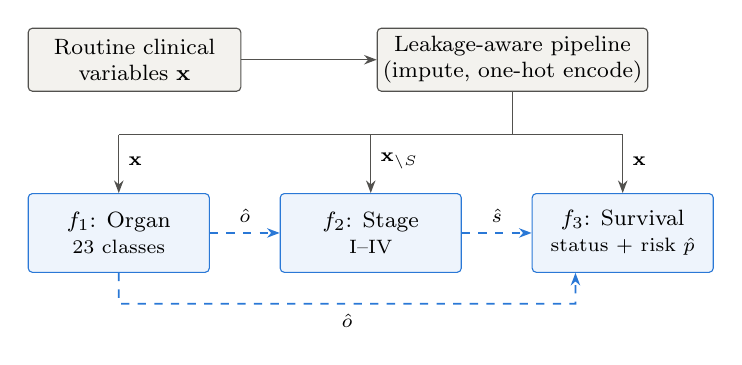
\begin{tikzpicture}[x=1mm,y=1mm,
  every node/.style={font=\footnotesize},
  box/.style={draw=vizink, fill=vizgray, rounded corners=1.5pt, align=center, inner sep=2pt, line width=0.4pt},
  mdl/.style={box, draw=vizblue, fill=vizblueL, minimum width=23mm, minimum height=10mm},
  arr/.style={-{Stealth[length=1.6mm]}, line width=0.5pt, draw=vizink},
  fb/.style={-{Stealth[length=1.6mm]}, line width=0.6pt, draw=vizblue, dashed}]
\node[box, minimum width=27mm, minimum height=8mm] (x) at (14,22) {Routine clinical\\variables $\mathbf{x}$};
\node[box, minimum width=34mm, minimum height=8mm] (pre) at (62,22) {Leakage-aware pipeline\\(impute, one-hot encode)};
\draw[arr] (x) -- (pre);
\node[mdl] (f1) at (12,0) {$f_1$: Organ\\{\scriptsize 23 classes}};
\node[mdl] (f2) at (44,0) {$f_2$: Stage\\{\scriptsize I--IV}};
\node[mdl] (f3) at (76,0) {$f_3$: Survival\\{\scriptsize status + risk $\hat p$}};
\draw[line width=0.5pt, draw=vizink] (pre.south) -- (62,12.5);
\draw[line width=0.5pt, draw=vizink] (12,12.5) -- (76,12.5);
\draw[arr] (12,12.5) -- (f1.north) node[pos=0.45, right, font=\scriptsize] {$\mathbf{x}$};
\draw[arr] (44,12.5) -- (f2.north) node[pos=0.45, right, font=\scriptsize] {$\mathbf{x}_{\setminus S}$};
\draw[arr] (76,12.5) -- (f3.north) node[pos=0.45, right, font=\scriptsize] {$\mathbf{x}$};
\draw[fb] (f1) -- node[above, font=\scriptsize] {$\hat o$} (f2);
\draw[fb] (f2) -- node[above, font=\scriptsize] {$\hat s$} (f3);
\draw[fb] (f1.south) -- (12,-9) -- node[below, font=\scriptsize] {$\hat o$} (70,-9) -- ([xshift=-6mm]f3.south);
\end{tikzpicture}
\caption{Cascaded framework. Each model receives the routine variables (the stage model receives them without stage and TNM, $\mathbf{x}_{\setminus S}$) plus the predictions of the preceding models (dashed).}
\label{fig:framework}
\end{figure}

\subsection{Preprocessing}
All preprocessing is part of a single pipeline fitted on training folds only, so no statistic of the test fold is used. Age is imputed with the median and standardised. Categorical variables with less than 5\% missing values (sex and morphology code) are imputed with the mode. Variables with more than 5\% missing values receive an explicit \emph{Unknown} level, so that structural missingness, such as an unstaged glioma, remains available as a signal. All categorical variables are one-hot encoded, and categories unseen during training are ignored at prediction time. The 101 patients flagged as age outliers by the interquartile-range rule (younger than 22.5 years) were retained, because they are genuine young patients with cancers typical of that age group rather than recording errors.

\subsection{Classifiers}
We compared logistic regression (LR), $k$-nearest neighbours (KNN), a support vector machine with RBF kernel (SVM)~\cite{cortes1995}, a decision tree (DT), random forest (RF, 300 trees)~\cite{breiman2001}, and three gradient-boosting libraries: XGBoost (XGB, 200 rounds)~\cite{chen2016}, LightGBM (LGBM, 300 rounds)~\cite{ke2017} and CatBoost~\cite{prokhorenkova2018}, together with a majority-class baseline, using scikit-learn~\cite{pedregosa2011}. Hyperparameter grids were: LR $C\in\{0.1,1,10\}$; KNN $k\in\{5,15,31\}$ with uniform or distance weights; SVM $C\in\{1,10\}$; DT maximum depth $\in\{\text{none},10,20\}$ and minimum leaf size $\in\{1,5\}$; RF minimum leaf size $\in\{1,3\}$ and feature fraction $\in\{\sqrt{d},0.2\}$; XGB depth $\in\{3,6\}$ and learning rate $\in\{0.1,0.3\}$; LGBM leaves $\in\{15,31\}$ and learning rate $\in\{0.05,0.1\}$. CatBoost used the fixed hyperparameters of our deployed models, because a single fit takes about a minute: for T2 and T3 it consumes the raw categories through its ordered target statistics (800 iterations, learning rate 0.05, depth 6), and for the 23-class T1, where per-class target statistics are prohibitively slow, it uses one-hot inputs (500 iterations, learning rate 0.1, depth 6).

\subsection{Evaluation protocol}
Performance was estimated with stratified 5-fold cross-validation repeated three times (15 outer folds). Within each outer training fold, hyperparameters of all learners except CatBoost were selected by a stratified 3-fold grid search maximising macro-F1, which keeps model selection separate from evaluation~\cite{cawley2010}. Because all three tasks are imbalanced, macro-F1 is the primary metric; we also report accuracy, balanced accuracy and, for T3, the area under the ROC curve (AUC), recall of the deceased class and the Brier score~\cite{brier1950}. Each model was compared with the best model of its task by the Nadeau--Bengio corrected resampled $t$-test~\cite{nadeau2003} ($\alpha=0.05$).

\subsection{Cascade analysis}
In the cascade, $f_2$ and $f_3$ receive a \emph{predicted} organ, whereas training data contain the true organ. To quantify the cost of this mismatch, we generated out-of-fold (OOF) organ predictions for every patient with a nested-tuned LR organ model, and evaluated $f_2$ and $f_3$ in four settings: (i) without any organ feature; (ii) with the true organ (an oracle upper bound); (iii) trained on the true organ but tested on the predicted organ (naive cascade); and (iv) trained and tested on OOF-predicted organs, so that the training distribution matches inference (OOF-consistent cascade).

\section{Results}
\begin{table*}[t]
\caption{Nested cross-validation results, mean\,$\pm$\,SD over 15 outer folds (\%; AUC as a fraction). Bold: best macro-F1 per task. $^{*}$Significantly lower macro-F1 than the best model (corrected resampled $t$-test, $p<0.05$). $^{\dagger}$Fixed, untuned hyperparameters.}
\label{tab:main}
\centering
\footnotesize
\setlength{\tabcolsep}{5pt}
\begin{tabular}{lccccccc}
\toprule
 & \multicolumn{2}{c}{T1: Organ (23 classes)} & \multicolumn{2}{c}{T2: Stage (4 classes)} & \multicolumn{3}{c}{T3: Survival (2 classes)} \\
\cmidrule(lr){2-3}\cmidrule(lr){4-5}\cmidrule(lr){6-8}
Model & Accuracy & Macro-F1 & Accuracy & Macro-F1 & Accuracy & Macro-F1 & AUC \\
\midrule
Majority class & 10.9\,$\pm$\,0.0 & 0.9\,$\pm$\,0.0 & 31.6\,$\pm$\,0.0 & 12.0\,$\pm$\,0.0 & 70.6\,$\pm$\,0.0 & 41.4\,$\pm$\,0.0 & -- \\
\midrule
Logistic regression & 94.4\,$\pm$\,0.3 & \textbf{93.7\,$\pm$\,0.4} & 52.8\,$\pm$\,1.3 & 49.5\,$\pm$\,1.2 & 78.3\,$\pm$\,1.0 & 72.4\,$\pm$\,1.1$^{*}$ & .838\,$\pm$\,.010 \\
$k$-nearest neighbours & 88.0\,$\pm$\,0.7 & 85.0\,$\pm$\,1.3$^{*}$ & 51.4\,$\pm$\,1.0 & 48.5\,$\pm$\,0.8$^{*}$ & 77.0\,$\pm$\,0.9 & 70.4\,$\pm$\,1.2$^{*}$ & .804\,$\pm$\,.018 \\
SVM (RBF) & 94.3\,$\pm$\,0.4 & 93.3\,$\pm$\,0.5 & 53.5\,$\pm$\,1.3 & \textbf{50.5\,$\pm$\,1.1} & 78.7\,$\pm$\,0.9 & 73.1\,$\pm$\,0.9$^{*}$ & .834\,$\pm$\,.011 \\
Decision tree & 91.5\,$\pm$\,0.7 & 89.8\,$\pm$\,0.9$^{*}$ & 49.3\,$\pm$\,1.6 & 45.7\,$\pm$\,1.7$^{*}$ & 76.5\,$\pm$\,0.9 & 71.6\,$\pm$\,0.7$^{*}$ & .788\,$\pm$\,.015 \\
Random forest & 92.6\,$\pm$\,0.6 & 91.1\,$\pm$\,0.7$^{*}$ & 52.5\,$\pm$\,1.2 & 50.2\,$\pm$\,1.1 & 78.9\,$\pm$\,1.1 & 73.3\,$\pm$\,1.3 & .839\,$\pm$\,.011 \\
XGBoost & 93.7\,$\pm$\,0.4 & 92.5\,$\pm$\,0.5$^{*}$ & 53.1\,$\pm$\,1.2 & 50.0\,$\pm$\,1.2 & 79.0\,$\pm$\,1.0 & 73.7\,$\pm$\,1.1 & .843\,$\pm$\,.009 \\
LightGBM & 92.4\,$\pm$\,0.6 & 90.0\,$\pm$\,0.8$^{*}$ & 51.4\,$\pm$\,1.2 & 49.2\,$\pm$\,1.1 & 78.9\,$\pm$\,0.9 & 73.6\,$\pm$\,1.0 & .843\,$\pm$\,.009 \\
CatBoost$^{\dagger}$ & 93.3\,$\pm$\,0.5 & 91.8\,$\pm$\,0.6$^{*}$ & 52.7\,$\pm$\,1.0 & 50.2\,$\pm$\,1.2 & 79.1\,$\pm$\,0.9 & \textbf{74.0\,$\pm$\,0.9} & .847\,$\pm$\,.010 \\
\bottomrule
\end{tabular}
\end{table*}

\subsection{Model comparison}
Table~\ref{tab:main} summarises the nested cross-validation. Every learner exceeded the majority baseline by a wide margin on all three tasks. For organ prediction, LR achieved the highest macro-F1 ($93.7\pm0.4$) and accuracy (94.4\%). The SVM was statistically indistinguishable (93.3, $p=0.12$), whereas all tree-based learners---XGBoost (92.5), CatBoost (91.8), RF (91.1), LightGBM (90.0) and DT (89.8)---and KNN (85.0) were significantly worse. For stage, the SVM was best (50.5), but LR, RF and the three boosting libraries were within 1.3 points and not significantly different. For survival, CatBoost obtained the highest macro-F1 (74.0) and AUC (0.847); XGBoost, LightGBM and RF were statistically indistinguishable from it, whereas LR trailed by 1.6 macro-F1 points and 0.009 AUC ($p=0.002$). No learner dominated across tasks, and the gap between LR and the best model never exceeded 1.6 macro-F1 points.

\subsection{Organ of origin}
\begin{table}[t]
\caption{Feature-group ablation for organ prediction (LR, 15 folds).}
\label{tab:ablation}
\centering
\footnotesize
\setlength{\tabcolsep}{4pt}
\begin{tabular}{lccc}
\toprule
Input variables & Acc. (\%) & Macro-F1 (\%) & $\Delta$F1 \\
\midrule
All routine variables & 94.4 & 93.7\,$\pm$\,0.4 & -- \\
\quad $-$ morphology code & 75.3 & 65.3\,$\pm$\,1.2 & $-$28.4 \\
\quad $-$ sex & 93.9 & 92.7\,$\pm$\,0.5 & $-$0.9 \\
\quad $-$ stage and TNM & 83.6 & 82.6\,$\pm$\,0.6 & $-$11.1 \\
\quad $-$ radiation, recurrence & 93.1 & 92.5\,$\pm$\,0.5 & $-$1.2 \\
Morphology code only & 74.5 & 73.5\,$\pm$\,0.6 & $-$20.1 \\
Age and sex only & 20.0 & 6.6\,$\pm$\,0.5 & $-$87.1 \\
\bottomrule
\end{tabular}
\end{table}

Table~\ref{tab:ablation} isolates the contribution of each variable group. Removing the morphology code reduced macro-F1 by 28.4 points, yet the code alone reached only 73.5, so the remaining variables carry complementary information. Stage and TNM fields contributed 11.1 points because their category sets, and the presence of an unstaged record, differ by cancer type. Sex added 0.9 points through sex-specific organs, and treatment and recurrence added 1.2. Age and sex alone were nearly uninformative (6.6).

\begin{figure}[t]
\centering
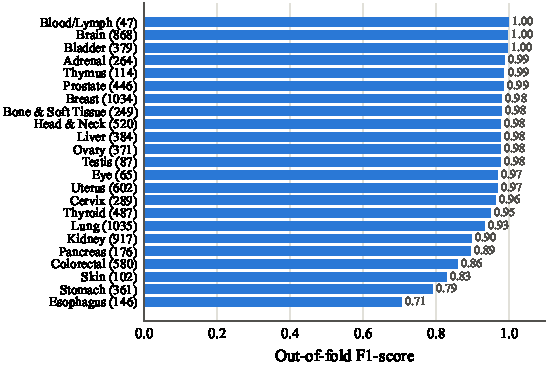
\includegraphics[width=\columnwidth]{figures/organ_f1.pdf}
\caption{Out-of-fold F1 per organ class for LR (first repetition); patient counts in parentheses.}
\label{fig:organ}
\end{figure}

Fig.~\ref{fig:organ} shows per-class performance: 15 of 23 classes reached an F1 of at least 0.95. The weakest were oesophagus (0.71), stomach (0.79), skin (0.83) and colorectal (0.86). The most frequent confusions were stomach$\rightarrow$colorectal and stomach$\rightarrow$lung, consistent with adenocarcinoma NOS (ICD-O-3 8140/3) being the most common morphology among oesophageal (59\%), stomach (39\%) and colorectal (85\%) patients. Error analysis further revealed that 243 patients (2.6\%) lacked a morphology code, and 242 of them had no clinical variable recorded at all because they had no match in the clinical table. The classifier necessarily assigns such empty records to a single class, and these 243 patients account for 162 of the 523 errors (31\%). On the 9,280 records with a morphology code, accuracy rises to 96.1\% and macro-F1 to 0.955.

\subsection{Stage}
\begin{figure}[t]
\centering
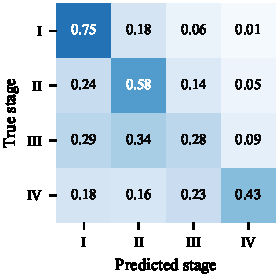
\includegraphics[width=0.62\columnwidth]{figures/stage_cm.pdf}
\caption{Row-normalised confusion matrix of the SVM stage model (out-of-fold, first repetition).}
\label{fig:stage}
\end{figure}

Stage is intrinsically hard without TNM. Fig.~\ref{fig:stage} shows that Stage~I is recognised best (recall 0.75), whereas Stage~III (0.28) and Stage~IV (0.43) are often assigned to earlier stages. Errors are ordinal: 66.8\% of misclassifications fall in an adjacent stage, and 84.7\% of all predictions lie within one stage of the truth. To quantify the leakage that our feature selection avoids, we retrained LR and LightGBM (the latter with the configuration of a TNM-based stage model built during development) with the T, N and M fields included: macro-F1 rose from 49.4 to 90.2 for LR and from 48.0 to 95.3 for LightGBM, an apparent gain that is entirely attributable to inputs that define the target. Adding the follow-up duration to T3 raised LR macro-F1 only from 72.5 to 73.3 but lifted the LightGBM AUC from 0.841 to 0.866, so flexible ensembles exploit leaked fields more aggressively than linear models.

\subsection{Survival and calibration}
\begin{figure}[t]
\centering
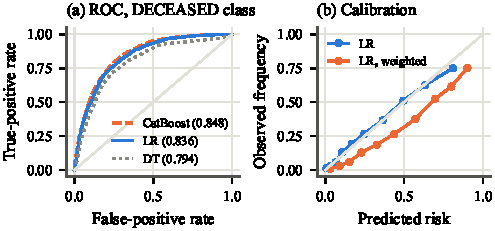
\includegraphics[width=\columnwidth]{figures/survival_roc_cal.pdf}
\caption{Survival prediction (out-of-fold, first repetition). (a) ROC curves with AUC in parentheses. (b) Calibration of LR with and without class weighting (deciles of predicted risk).}
\label{fig:surv}
\end{figure}

LR and the ensembles produced almost identical ROC curves (Fig.~\ref{fig:surv}a). Calibration was good throughout: Brier scores were 0.142 for CatBoost, 0.143 for LightGBM, 0.144 for XGBoost, 0.145 for RF and 0.146 for LR (Fig.~\ref{fig:surv}b), far below the 0.294 of the baseline. At the default 0.5 threshold, however, only 55--60\% of deceased patients were identified. Class-weighted LR raised the recall of the deceased class to 77.1\% and balanced accuracy from 71.4\% to 76.3\% without changing the AUC (0.839), but it worsened the Brier score to 0.165 and systematically overestimated risk. When a risk percentage is shown to users, adjusting the decision threshold is therefore preferable to reweighting the training loss.

\subsection{Cascade error propagation}
\begin{table}[t]
\caption{Effect of the organ input on downstream tasks (LR, 15 folds, \%; AUC as a fraction).}
\label{tab:cascade}
\centering
\footnotesize
\setlength{\tabcolsep}{3.5pt}
\begin{tabular}{lcccc}
\toprule
 & \multicolumn{2}{c}{T2: Stage} & \multicolumn{2}{c}{T3: Survival} \\
\cmidrule(lr){2-3}\cmidrule(lr){4-5}
Organ input & Acc. & Macro-F1 & Macro-F1 & AUC \\
\midrule
(i) No organ feature & 50.1 & 45.7 & 71.5 & 0.830 \\
(ii) True organ (oracle) & 52.8 & 49.5 & 72.4 & 0.838 \\
(iii) Cascade, naive & 53.1 & 49.6 & 72.2 & 0.835 \\
(iv) Cascade, OOF-consistent & 53.2 & 49.8 & 72.1 & 0.836 \\
\bottomrule
\end{tabular}
\end{table}

The OOF organ predictions used in the cascade were 94.2\% accurate. Table~\ref{tab:cascade} shows that the organ feature improves stage macro-F1 from 45.7 to 49.5 and survival AUC from 0.830 to 0.838. Replacing the true organ by the predicted one caused no measurable loss: the naive cascade (49.6; 0.835) and the OOF-consistent cascade (49.8; 0.836) both matched the oracle within fold-to-fold variation. Two factors explain this robustness. The records without clinical data, which cause a third of all organ errors, are excluded from T2 and T3 by construction, so the organ model is correct for 95.0\% of the stage cohort and 96.1\% of the survival cohort. In addition, the downstream models receive the morphology code directly, which carries much of the same information as the organ label. OOF-consistent training gave no further gain, so the simpler naive cascade is adequate in this setting.

\subsection{Deployment}
The fitted pipelines (preprocessing and model) are serialised and served by a Flask web application; any field can be left as \emph{Unknown}, which the pipeline maps to the same missingness category seen in training. The current deployment uses CatBoost for organ and survival. Trained once on an 80\% split and evaluated on the remaining 20\%, these models reached 92.7\% organ accuracy (macro-F1 0.907) and a survival AUC of 0.864 (macro-F1 0.765). The survival figure lies above the cross-validated $0.847\pm0.010$, which illustrates how far a single split can deviate from a repeated estimate. On a consumer laptop, prediction takes a median of 9.9\,ms per patient for the two CatBoost models and 19.7\,ms for the complete LR cascade.

\section{Discussion}
\subsubsection*{Linear versus boosted models}
Across three tasks and 15 outer folds, regularised LR was the best organ classifier, significantly ahead of all five tree-based learners, and within 1.6 macro-F1 points of the best model elsewhere, in line with systematic evidence that ML rarely outperforms LR for clinical prediction~\cite{christodoulou2019}. One-hot morphology and staging categories make the organ classes nearly linearly separable, which removes the main advantage of tree ensembles on tabular data~\cite{grinsztajn2022}. Gradient boosting helped only for survival, where CatBoost's native handling of high-cardinality categories gave the best discrimination and calibration. We therefore recommend LR for organ and stage, where it is as accurate and fully interpretable~\cite{rudin2019}, and CatBoost for survival when its 0.009 AUC gain justifies a less transparent model.

\subsubsection*{Clinical interpretation}
The organ model largely recovers the mapping from morphology and staging conventions to anatomical site. This is useful for registry quality control (flagging records whose coded site disagrees with the prediction), for triage, and as a prior where molecular or imaging work-up is unavailable. It does not solve cancer of unknown primary: TCGA contains primary tumours with known sites, and many morphology codes are site-specific. Stage prediction without TNM should be read as a coarse estimate; its value lies in its ordinal errors and in filling missing values for the downstream survival model.

\subsubsection*{Limitations}
All data come from a single consortium of mainly US academic centres, and no external validation was possible. Vital status is a binary endpoint that ignores censoring and unequal follow-up~\cite{liu2018}; time-to-event models such as random survival forests~\cite{ishwaran2008} are a natural extension. The morphology code may not be available before pathology review, which limits use at the earliest point of care. Finally, race and ethnicity were excluded, but performance was not audited across demographic subgroups.

\section{Conclusion}
We presented a leakage-aware cascade that predicts organ of origin, AJCC stage and vital status from routine clinical variables of 9,523 TCGA patients. Under nested, repeated cross-validation of eight classifiers, logistic regression identified the organ with 94.4\% accuracy, significantly ahead of all tree ensembles, while CatBoost gave the best survival discrimination (AUC 0.847) with logistic regression close behind (0.838). Explicit leakage control proved essential: including TNM fields inflated stage macro-F1 from about 0.49 to 0.90--0.95, and cascading predicted organ labels caused no loss. Future work will add external validation, time-to-event modelling, fairness auditing and the free-text pathology reports of TCGA-Reports~\cite{kefeli2024}.

\section*{Data and Code Availability}
TCGA clinical data are publicly available through cBioPortal, and TCGA-Reports is available from its authors~\cite{kefeli2024}. The code reproducing every experiment, table and figure is available at \{repository URL\}.

\IEEEtriggeratref{25}
\begin{thebibliography}{30}
\small

\bibitem{varadhachary2014}
G.~R. Varadhachary and M.~N. Raber, ``Cancer of unknown primary site,'' \emph{N. Engl. J. Med.}, vol.~371, no.~8, pp. 757--765, 2014.

\bibitem{amin2017}
M.~B. Amin \emph{et al.}, ``The eighth edition AJCC cancer staging manual: Continuing to build a bridge from a population-based to a more `personalized' approach to cancer staging,'' \emph{CA Cancer J. Clin.}, vol.~67, no.~2, pp. 93--99, 2017.

\bibitem{cruz2006}
J.~A. Cruz and D.~S. Wishart, ``Applications of machine learning in cancer prediction and prognosis,'' \emph{Cancer Inform.}, vol.~2, pp. 59--77, 2006.

\bibitem{kourou2015}
K.~Kourou, T.~P. Exarchos, K.~P. Exarchos, M.~V. Karamouzis, and D.~I. Fotiadis, ``Machine learning applications in cancer prognosis and prediction,'' \emph{Comput. Struct. Biotechnol. J.}, vol.~13, pp. 8--17, 2015.

\bibitem{grewal2019}
J.~K. Grewal \emph{et al.}, ``Application of a neural network whole transcriptome-based pan-cancer method for diagnosis of primary and metastatic cancers,'' \emph{JAMA Netw. Open}, vol.~2, no.~4, p. e192597, 2019.

\bibitem{penson2020}
A.~Penson \emph{et al.}, ``Development of genome-derived tumor type prediction to inform clinical cancer care,'' \emph{JAMA Oncol.}, vol.~6, no.~1, pp. 84--91, 2020.

\bibitem{jiao2020}
W.~Jiao \emph{et al.}, ``A deep learning system accurately classifies primary and metastatic cancers using passenger mutation patterns,'' \emph{Nat. Commun.}, vol.~11, art. no. 728, 2020.

\bibitem{lu2021}
M.~Y. Lu \emph{et al.}, ``AI-based pathology predicts origins for cancers of unknown primary,'' \emph{Nature}, vol.~594, pp. 106--110, 2021.

\bibitem{fritz2000}
A.~Fritz \emph{et al.}, Eds., \emph{International Classification of Diseases for Oncology}, 3rd~ed. Geneva, Switzerland: World Health Organization, 2000.

\bibitem{kaufman2012}
S.~Kaufman, S.~Rosset, C.~Perlich, and O.~Stitelman, ``Leakage in data mining: Formulation, detection, and avoidance,'' \emph{ACM Trans. Knowl. Discov. Data}, vol.~6, no.~4, art. no. 15, 2012.

\bibitem{kapoor2023}
S.~Kapoor and A.~Narayanan, ``Leakage and the reproducibility crisis in machine-learning-based science,'' \emph{Patterns}, vol.~4, no.~9, art. no. 100804, 2023.

\bibitem{cawley2010}
G.~C. Cawley and N.~L.~C. Talbot, ``On over-fitting in model selection and subsequent selection bias in performance evaluation,'' \emph{J. Mach. Learn. Res.}, vol.~11, pp. 2079--2107, 2010.

\bibitem{christodoulou2019}
E.~Christodoulou \emph{et al.}, ``A systematic review shows no performance benefit of machine learning over logistic regression for clinical prediction models,'' \emph{J. Clin. Epidemiol.}, vol.~110, pp. 12--22, 2019.

\bibitem{hoadley2018}
K.~A. Hoadley \emph{et al.}, ``Cell-of-origin patterns dominate the molecular classification of 10,000 tumors from 33 types of cancer,'' \emph{Cell}, vol.~173, no.~2, pp. 291--304, 2018.

\bibitem{delen2005}
D.~Delen, G.~Walker, and A.~Kadam, ``Predicting breast cancer survivability: A comparison of three data mining methods,'' \emph{Artif. Intell. Med.}, vol.~34, no.~2, pp. 113--127, 2005.

\bibitem{agrawal2012}
A.~Agrawal, S.~Misra, R.~Narayanan, L.~Polepeddi, and A.~Choudhary, ``Lung cancer survival prediction using ensemble data mining on SEER data,'' \emph{Sci. Program.}, vol.~20, no.~1, pp. 29--42, 2012.

\bibitem{ishwaran2008}
H.~Ishwaran, U.~B. Kogalur, E.~H. Blackstone, and M.~S. Lauer, ``Random survival forests,'' \emph{Ann. Appl. Stat.}, vol.~2, no.~3, pp. 841--860, 2008.

\bibitem{katzman2018}
J.~L. Katzman \emph{et al.}, ``DeepSurv: Personalized treatment recommender system using a Cox proportional hazards deep neural network,'' \emph{BMC Med. Res. Methodol.}, vol.~18, art. no. 24, 2018.

\bibitem{liu2018}
J.~Liu \emph{et al.}, ``An integrated TCGA pan-cancer clinical data resource to drive high-quality survival outcome analytics,'' \emph{Cell}, vol.~173, no.~2, pp. 400--416, 2018.

\bibitem{nadeau2003}
C.~Nadeau and Y.~Bengio, ``Inference for the generalization error,'' \emph{Mach. Learn.}, vol.~52, no.~3, pp. 239--281, 2003.

\bibitem{collins2024}
G.~S. Collins \emph{et al.}, ``TRIPOD+AI statement: Updated guidance for reporting clinical prediction models that use regression or machine learning methods,'' \emph{BMJ}, vol.~385, p. e078378, 2024.

\bibitem{vancalster2019}
B.~Van~Calster \emph{et al.}, ``Calibration: The Achilles heel of predictive analytics,'' \emph{BMC Med.}, vol.~17, art. no. 230, 2019.

\bibitem{grinsztajn2022}
L.~Grinsztajn, E.~Oyallon, and G.~Varoquaux, ``Why do tree-based models still outperform deep learning on typical tabular data?'' in \emph{Adv. Neural Inf. Process. Syst. (NeurIPS), Datasets and Benchmarks Track}, 2022.

\bibitem{rudin2019}
C.~Rudin, ``Stop explaining black box machine learning models for high stakes decisions and use interpretable models instead,'' \emph{Nat. Mach. Intell.}, vol.~1, no.~5, pp. 206--215, 2019.

\bibitem{kefeli2024}
J.~Kefeli and N.~Tatonetti, ``TCGA-Reports: A machine-readable pathology report resource for benchmarking text-based AI models,'' \emph{Patterns}, vol.~5, no.~3, art. no. 100933, 2024.

\bibitem{cerami2012}
E.~Cerami \emph{et al.}, ``The cBio cancer genomics portal: An open platform for exploring multidimensional cancer genomics data,'' \emph{Cancer Discov.}, vol.~2, no.~5, pp. 401--404, 2012.

\bibitem{cortes1995}
C.~Cortes and V.~Vapnik, ``Support-vector networks,'' \emph{Mach. Learn.}, vol.~20, no.~3, pp. 273--297, 1995.

\bibitem{breiman2001}
L.~Breiman, ``Random forests,'' \emph{Mach. Learn.}, vol.~45, no.~1, pp. 5--32, 2001.

\bibitem{chen2016}
T.~Chen and C.~Guestrin, ``XGBoost: A scalable tree boosting system,'' in \emph{Proc. 22nd ACM SIGKDD Int. Conf. Knowl. Discov. Data Min.}, 2016, pp. 785--794.

\bibitem{ke2017}
G.~Ke \emph{et al.}, ``LightGBM: A highly efficient gradient boosting decision tree,'' in \emph{Adv. Neural Inf. Process. Syst. (NeurIPS)}, vol.~30, 2017, pp. 3146--3154.

\bibitem{prokhorenkova2018}
L.~Prokhorenkova, G.~Gusev, A.~Vorobev, A.~V. Dorogush, and A.~Gulin, ``CatBoost: Unbiased boosting with categorical features,'' in \emph{Adv. Neural Inf. Process. Syst. (NeurIPS)}, vol.~31, 2018.

\bibitem{pedregosa2011}
F.~Pedregosa \emph{et al.}, ``Scikit-learn: Machine learning in Python,'' \emph{J. Mach. Learn. Res.}, vol.~12, pp. 2825--2830, 2011.

\bibitem{brier1950}
G.~W. Brier, ``Verification of forecasts expressed in terms of probability,'' \emph{Mon. Weather Rev.}, vol.~78, no.~1, pp. 1--3, 1950.

\end{thebibliography}


\end{document}
